\newpage
\section{Линейное нормированное пространство $C(K)$ для компактного метрического пространства $(K, \rho)$, его полнота. Критерий Арцела-Асколи вполне ограниченности подмножества пространства $C(K)$.}
\begin{definition}
	Пространство $C(K)$ --- множество непрерывных на компакте $K$ функций $f : K \rr \R$ по умолчанию имеет норму:
	$$
	\|f\|_c  = \sup\limits_{x \in K} |f(x)| = \max\limits_{x \in K}|f(x)|
	$$
\end{definition}
\begin{theorem}[Арцела-Асколи]\label{th:arzela}
	Пусть $(K, \rho)$ --- компактное метрическое пространство. Тогда $S \subset C(K)$ --- вполне ограниченно тогда и только тогда когда
	\begin{enumerate}
		\item $S$ --- ограниченно в $C(K)$, то есть $\exists R > 0 \forall f \in S \Rightarrow \|f\|_c \leq R$
		\item $S$ --- равностепенно непрерывно: 
		$$
		\forall \eps > 0 \exists \delta = \delta(\eps): \forall f \in S, \ \forall x, y \in K : \rho(x,y) \leq \delta \Rightarrow |f(x) - f(y)| \leq \eps 
		$$
	\end{enumerate}
\end{theorem}
\begin{proof}
	Необходимость. $S$ --- вполне ограниченно $\Rightarrow$ $S$ --- ограниченно. Имеем конечную $\eps$-сеть:
	$$
	\forall \eps > 0 \exists f_1, \dots, f_M \in S: \ S \subset \bigcup_{m = 1}^M B_\eps(f_m)
	$$
	Тогда по теореме кантора, функции $f_m$ равномерно непрерывны на $K$:
	$$
	\forall m \in \overline{1, M} \ \exists \delta_m(\eps) > 0 : \ \forall x,y \in K \ \rho(x,y) \leq \delta_m \Rightarrow |f_m(x) - f_m(y)| \leq \eps 
	$$
	Тогда положив $\delta = \min\limits_{m \in \overline{1, M}} \delta_m$ получим, что $\delta$ зависит только от $\eps$ и 
	$$
	\forall m \in \overline{1, M}, \ \forall x,y \in K:  \rho(x,y) < \delta \Rightarrow |f_m(x) - f_m(y)| \leq \eps 
	$$
	Тогда, пользуясь неравенством треугольника, получаем:
	$$
	\begin{gathered}
		\forall f \in S: \exists m \in \overline{1, M}: f \in B_\eps(f_m) \Rightarrow \forall x,y \in K, \ \rho(x,y) < \delta: \\ \ |f(x) - f(y)| \leq |f(x) - f_m(x)| + |f_m(x) - f_m(y)| + |f_m(y) - f(y)| \leq \eps + \eps + \eps = 3\eps
	\end{gathered}
	$$
	Таким образом необходимость доказана. Докажем достаточность. Пусть выполнено:
	\begin{enumerate}
		\item $S$ --- ограниченно в $C(K)$, то есть $\exists R > 0 \forall f \in S \Rightarrow \|f\|_c \leq R$
		\item $S$ --- равностепенно непрерывно: 
		$$
		\forall \eps > 0 \exists \delta = \delta(\eps): \forall f \in S, \ \forall x, y \in K : \rho(x,y) \leq \delta \Rightarrow |f(x) - f(y)| \leq \eps 
		$$
	\end{enumerate}
	Для числа $\delta(\eps)$ в компактом метрическом пространстве $(K, \rho)$ мы имеем конечную $\delta(\eps)$-сеть:
	$$
	x_1, \dots, x_M \in K: K = \bigcup_{m=1}^M B^K_{\delta(\eps)}(x_m) 
	$$
	Тогда построим:
	$$
	S_\eps = \{(f(x_1), \dots f(x_M)) \in \R^M \mid f \in S\}
	$$
	Тогда в силу ограниченности $S$:
	$$
	S_\eps \subset P_R = \{(z_1, \dots, z_M) \in R^M \mid \forall n \in \overline{1, M}: |z_n| \leq R \}
	$$
	Режем данный кубик на кубики со стороной не больше $\eps$.
	\begin{figure}[h!]
		\centering
		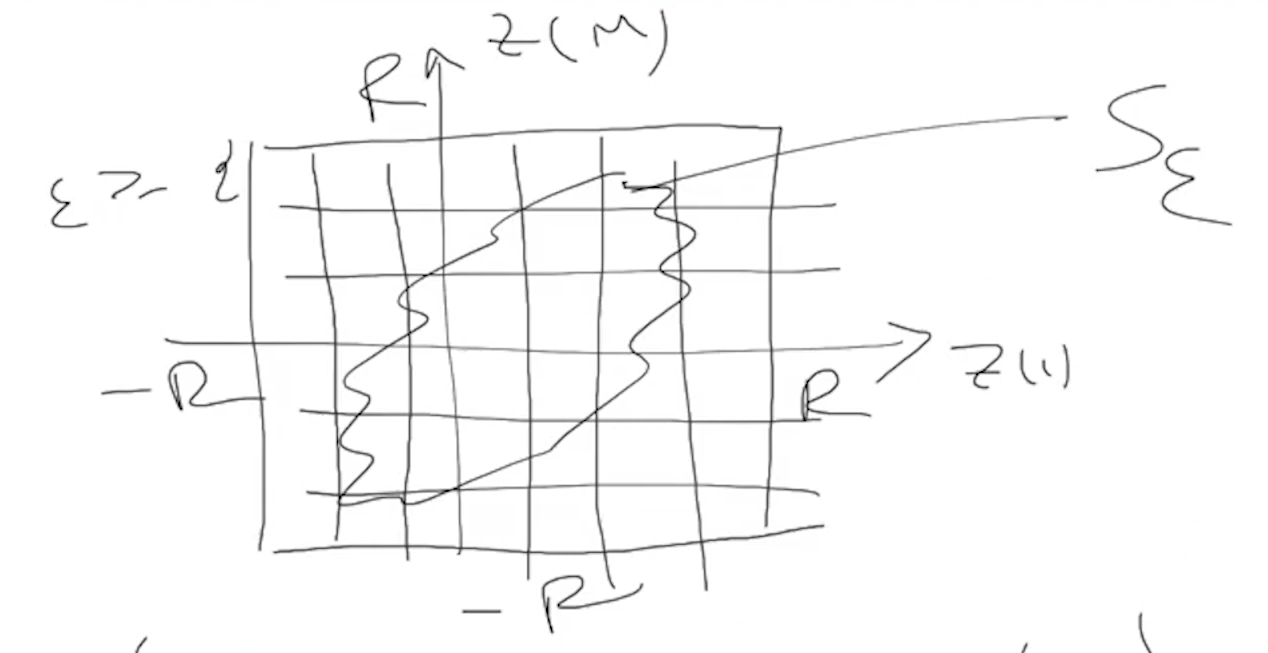
\includegraphics[width=0.7\linewidth]{pic/screenshot001}
		\caption{}
		\label{fig:screenshot001}
	\end{figure}

	Обозначим $\square$ --- элементарный кубик, рассмотрим: $G = \{\square : \square \cap S_\eps \neq \varnothing \}$ этих кубиков конечное число и $\forall \square \in G \ \exists f_\square \in S$ такая что 
	$$
	\begin{pmatrix}
		f_\square(x_1) \\
		\vdots \\
		f_\square(x_M)
	\end{pmatrix} \in \square \cap S_\eps \neq \varnothing
	$$  тогда рассматриваем соответствующие $C_\eps = \{f_\square \in S \mid \square \in G\}$ --- их тоже конечно. Тогда
	$$
	\forall f \in S: (f(x_1), \dots, f(x_M)) \in S_\eps \subset P_R \Rightarrow \exists f_\square: \forall m \in \overline{1, M}: |f(x_m) - f_\square(x_m)| \leq \eps
	$$
	Тогда 
	$$\forall x \in K 	\ \exists m \in \overline{1, M}: \ x \in B_{\delta(\eps)}^K(x_m)$$
	То есть $\rho(x,x_m) \leq \delta(\eps)$ и тогда
	$$
	|f(x) - f_\square(x)| \leq |f(x) - f(x_m)| + |f(x_m) - f_\square(x_m)| + |f_\square(x_m) - f_\square(x)| \leq 3\eps \Rightarrow \|f - f_\square\|_c \leq 3\eps
	$$
	Таким образом $S$ --- вполне ограниченно. 
\end{proof}
